\chapter{\textit{Microplanning}}
\label{cap:microplanning}

La etapa de \textit{microplanning} será la encargada de, a partir del \textit{document plan} producido por la etapa anterior, producir una especificación más detallada del el texto a generar. 

En éste capítulo presentaremos las tres tareas que, según Reiter y Dale~\cite{reiter_dale}, deberían llevarse a cabo en esta etapa: lexicalización, agregación y generación de expresiones de referencia. Luego definiremos en detalle la entrada y salida del \textit{microplanner}. Finalmente profundizaremos particularmente sobre la tarea de lexicalización que debemos llevar a cabo para este trabajo.

A lo largo de este capítulo continuaremos con el ejemplo utilizado en la etapa anterior, ilustrando cómo a partir del \textit{document plan} presentado en la la figura \ref{fig:png_document_plan_ej} construiremos una especificación más detallada del documento a generar.

\section{Tareas del \textit{Microplanner}}

Como mencionamos previamente, el \textit{microplanner} será el encargado de transformar el \textit{document plan} generado en la etapa anterior en una especificación más refinada del texto a generar. Cabe aclarar que el resultado de esta etapa no será todavía el texto final ya que quedarán por tomar decisiones acerca de la sintaxis, morfología y cuestiones de presentación, de las cuales se encargará el realizador de superficie.

Como mencionamos en el capítulo~\ref{cap:nlg_intro}, dentro de las tareas generalmente realizadas por el \emph{microplanner} podemos destacar las siguientes:

\medskip
\noindent
\textbf{Lexicalización:} esta tarea se encarga de elegir qué palabras particulares y qué constructores sintácticos usar para comunicar la información contenida en el \textit{document plan}. Desarrollaremos más en detalle el trabajo realizado por esta etapa en la sección~\ref{sec:microplanning_lexicalization}


\medskip
\noindent
\textbf{Agregación:} la función de esta tarea es la de combinar los elementos informativos del \emph{document plan} con el fin de conseguir un texto más fluido y legible. La agregación decide qué elementos se pueden agrupar para generar oraciones generalmente más complejas sin modificar el significado de las mismas. Por ejemplo, consideremos las siguientes dos descripciones posibles para la clase de prueba \emph{LookUp\_SP\_1} (figura \ref{fig:ej_corpus}):


\begin{center}
\begin{enumerate}
  \item \emph{El símbolo a buscar pertenece a los símbolos cargados en la tabla. El símbolo a buscar es el único elemento de los símbolos cargados en la tabla.} 
  \item \emph{El símbolo a buscar pertenece a los símbolos cargados en la tabla y éste es el único elemento de los símbolos cargados en la tabla.}
\end{enumerate}
\end{center}

\medskip
\noindent
Para este trabajo, decidimos expresar nuestras descripciones siguiendo el estilo de la primer frase del ejemplo anterior, por lo cual nuestro \textit{microplanner} no realizará tareas de agregación. En nuestro caso en particular creemos que será útil para el lector que cada oración de una descripción haga referencia a una única restricción del esquema de la clase de prueba. De esta forma podríamos identificar con mayor facilidad cuál es la descripción para cada expresión particular de una clase de prueba.


\medskip
\noindent
\textbf{Generación de expresiones de referencia:} esta tarea se encarga de determinar qué frases deben ser usadas para identificar las diferentes menciones al mismo elemento en un texto a fin de aportar fluidez a éste. Más específicamente, en los casos que se hace referencia a una entidad que ya ha aparecido en el texto se puede remplazar la misma por otra frase que la referencie. La elección de qué expresión utilizar para referirse a la entidad dependerá del contexto y deberá hacerse sin introducir ambigüedad para el lector. Por ejemplo, en la segunda alternativa presentada anteriormente para describir la clase de prueba \emph{LookUp\_SP\_1}:

\begin{center}
 \emph{\textbf{El símbolo a buscar} pertenece a los símbolos cargados en la tabla y \textbf{éste} es el único elemento de los símbolos cargados en la tabla.}
\end{center}

\noindent
Reemplazamos la segunda ocurrencia de ``el símbolo a buscar'' por el pronombre ``éste''.

\smallskip
Al igual que la tarea de agregación, la generación de expresiones de referencia excede el alcance de este trabajo y  nuestro \textit{microplanner} no realizará tareas este tipo. Sin embargo, en el capítulo \ref{cap:conclusion} propondremos, como un posible trabajo a futuro, la inclusión de las tareas agregación y generación de expresiones de referencia a nuestro sistema. 

%TODO en trabajo futuro se puede relacionar la agregacion con generacion de expresiones de referencia. Diciendo que la inclusion de tareas de agregacion probablemente requieran tareas de generacion de expresiones de referencia para la generacion de textos más fluidos.


\section{Entrada y salida del \textit{microplanner}}
La entrada del \textit{microplanner} será un \textit{document plan} producido por la etapa anterior. Observemos por ejemplo el \textit{document plan} presentado en la figura \ref{fig:png_document_plan_ej} del capítulo anterior, utilizado para modelar la descripción de la clase de prueba \emph{LookUp\_SP\_1}. Esta abstracción no especifica las frases que nuestro sistema debe generar, ni si deben estar enumeradas en una lista de ítems o agrupadas en secciones, por ejemplo. Necesitaremos una especificación más concreta, un modelo más detallado del documento y de las frases a generar. Será entonces responsabilidad del \textit{microplanner}  construir a partir del \textit{document plan} una especificación más concreta del texto a generar.

Llamaremos especificación del texto a la especificación resultado de esta etapa. Ésta se encargará de modelar los distintos elementos que compondrán el texto final (como párrafos, lista de ítems, etc.). Esta especificación estará compuesta en base a especificaciones de frase encargadas de modelar las distintas oraciones que serán incluidas en el texto final (veremos que cada una de estas se construirán a partir de los mensajes contenidos en el \textit{document plan}). Será luego tarea de la siguiente etapa convertir los nodos internos de la especificación del texto en anotaciones especificas para el sistema de presentación\footnote{Llamamos sistemas de presentación a los sistemas encargados de post-procesar las anotaciones antes mencionadas y presentarle al usuario el documento de manera apropiada. Por ejemplo, \LaTeX, Microsoft Word o web browsers como Firefox o Chrome son algunos de los posibles sistemas de presentación.} (realización de estructura) y transformar las especificaciones de frase en oraciones o frases sintáctica, morfológica y ortográficamente correctas (realización lingüística). 

%para que luego, en la etapa de realización de superficie podamos generar el texto final en base a los requerimientos analizados en el capítulo \ref{cap:corpus}. 

En lo que queda de esta sección estudiaremos cómo se encuentra constituida nuestra especificación del texto, describiendo también cómo están formadas nuestras especificaciones de frase.

\subsection{Especificación del texto}

%TODO faltaría explayar un poco más y hablar sobre conceptos de phrase y text specification
%Como vimos en el capítulo anterior, la salida del  \textit{document planner} es una estructura donde se encuentran agrupados los elementos informativos que deseamos comunicar. Estos elementos o \emph{mensajes} contenidos en el \emph{document plan} especifican de una manera abstracta la información que debemos comunicar en el texto final, pero no especifican, por ejemplo, que palabras debemos usar para hacerlo. 

%Será el \textit{microplanner} el encargado de tomar este tipo de decisiones. Éste tomará como entrada un \textit{document plan} y deberá producir una especificación más refinada del texto que deseamos generar, la cual será utilizada luego por el \emph{realizador de superficie} para producir el texto final.

La especificación de texto para nuestro sistema, deberá caracterizar la estructura del documento final que nuestro sistema debe producir. Es por esto que modelaremos los mismos utilizando un árbol, donde los hojas especificarán las frases u oraciones a generar (las especificaciones de frase), y los nodos internos establecerán cómo estas frases tendrán que ser agrupadas en elementos del documento (como párrafos, secciones, lista de ítems, etc). 

La estructura de los documentos que debemos generar en este trabajo resulta relativamente simple. Como vimos en el capítulo \ref{cap:corpus}, los documentos de descripciones poseen un título y luego se detallan una por una las descripciones de las distintas clases de prueba, donde para cada una de éstas aparece el nombre de la clase de prueba, junto a una pequeña descripción de la operación a testear y luego una lista de ítems que describirán cada una de las restricciones pertenecientes a la clase de prueba que se describe. Es por esto que para este trabajo utilizaremos sólo dos elementos para modelar la estructura interna del documento \emph{TSDocumento} y \emph{TSListaItems}:

\medskip
\noindent
\textbf{TSDocumento:} modela el documento final, por lo tanto solo tendremos un elemento de este tipo en nuestra especificación del texto y éste será la raíz del documento. Éste elemento contendrá información general sobre el documento, como el título y una especificación para cada descripción de clase de prueba, modeladas mediante \emph{TSListaItems}.

\medskip
\noindent
\textbf{TSListaItems:} modela el texto que describirá a una clase de prueba. Este elemento contiene una especificación de frase que modelará el texto correspondiente al título y al detalle de la descripción. Además contendrá una lista de especificaciones de frase que especificarán las frases para cada una de las verbalizaciones de las expresiones contenidas en la clase de prueba en cuestión. Habrá una \emph{TSListaItems} por cada clase de prueba a describir.

\begin{figure}[H]
  	\centering
	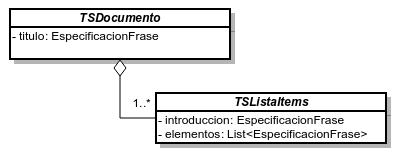
\includegraphics[scale=0.3]{img/text_spec.png}
	\caption{Especificación de texto.}
  	\label{fig:text_spec}
\end{figure}

En la figura anterior podemos observar la estructura abstracta que tendrán nuestras especificaciones del texto y por ejemplo, sin meternos en detalle todavía sobre la estructura de las especificaciones de frase, en la figura \ref{fig:text_spec_ej} podemos ver una especificación de frase para el ejemplo introducido anteriormente (página \pageref{fig:ej_corpus}).

\begin{figure}[H]
  	\centering
	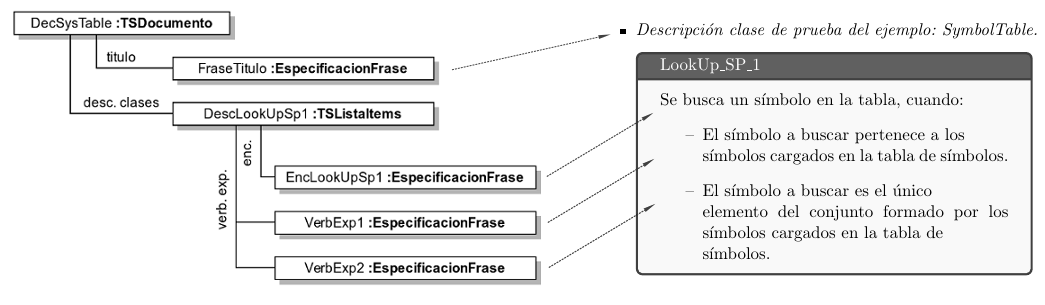
\includegraphics[scale=0.35]{img/ej_text_spec.png}
	\caption{Ejemplo especificación del texto.}
  \label{fig:text_spec_ej}
\end{figure}

Veremos en el próximo capítulo cómo, en la etapa de realización estructural, transformaremos estos elementos en anotaciones para el sistema de presentación.

\subsection{Especificación de frase}

En la literatura sobre NLG podemos encontrar muchas alternativas en lo que respecta a la especificación de frases (\textit{skeletal propositions}, \textit{meaning specifications} y \textit{lexicalised case frames} entre otras \cite{reiter_dale}). Todas éstas varían en el nivel de abstracción que poseen. Las representaciones más abstractas le darán más flexibilidad a las etapas de \textit{document planning} y \textit{microplanning}, pero al mismo tiempo nos obligarán a tener un realizador de superficie más sofisticado. Por otro lado, las especificaciones menos abstractas, requieren que el \textit{document planner} y el \textit{microplanner} realicen un mayor trabajo, pero también tendrán más control sobre el texto a producir. Uno de los objetivos que tuvimos a la hora de idear una estructura para nuestra especificación de frases fue que ésta sea independiente de nuestro problema; pretendemos que hable en términos de la lengua (castellano en nuestro caso) que queremos generar y no en términos específicos de Z. Es por esto que decidimos especificar las oraciones a generar mediante árboles sintácticos, donde los constituyentes de éstos son los sintagmas de la oración que deseamos generar. Esto le dará la posibilidad al realizador lingüístico de poder identificar la función de cada uno de los constituyentes de la oración. Por ejemplo, como detallamos en los requerimientos de la sección \ref{sec:corpus_gramatica}, el \emph{realizador de superficie} necesitará identificar el núcleo de un sintagma nominal (núcleo del sujeto) para poder producir una oración en la que haya concordancia de número y persona entre el verbo y el sujeto. Como consecuencia del ejemplo anterior, nuestro realizador lingüístico deberá proveerle al realizador de superficie una especificación que permita identificar el sujeto, predicado y verbo de una oración. Creemos que con los elementos presentes en la figura~\ref{fig:phase_spec} podremos modelar la frases incluidas en el corpus.

\begin{figure}[h]
  	\centering
	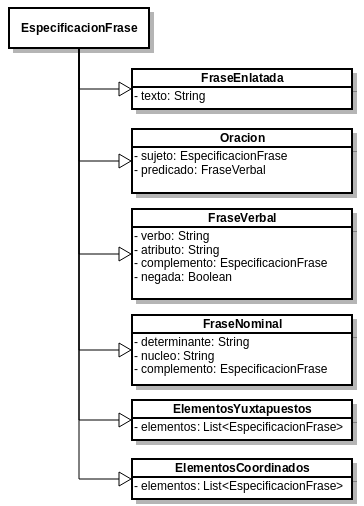
\includegraphics[scale=0.7]{img/phrase_spec.png}
	\caption{Especificación de frase.}
  	\label{fig:phase_spec}
\end{figure}

No pretendemos modelar toda la lengua castellana con estos elementos sino solo un subconjunto que nos provea las herramientas necesarias para permitirle al \emph{realizador de superficie} generar las frases definidas en el capítulo \ref{sec:corpus_analisis}, ya que el desarrollo de un realizador lingüístico que considere todas las construcciones sintácticas de nuestra lengua escapa el alcance de este trabajo. Es por esto que sólo modelamos los sintagmas nominales (FraseNominal) y verbales (FraseVerbal) y nos vemos obligados a incluir otros elementos como ElementosYuxtapuestos para salvaguardar la falta de algunos constituyentes sintácticos como sintagmas adjetivales, preposicionales, etc. 

A continuación describiremos brevemente cada uno de estos elementos, profundizando sobre la realización de los mismos en el capítulo \ref{cap:linguistic_realization}.


\medskip
\begin{itemize}
\item{\emph{\textbf{FraseEnlatada}}: Representa texto que no necesita ningún tipo de procesamiento posterior a realizar durante la realización lingüística, será incluido en el texto tal cual fue establecido.}
\item{\emph{\textbf{Oracion}}: Modela oraciones bimembres. El realizador lingüístico deberá procesarlas en base a una serie de reglas gramaticales para producir un texto sintáctica, morfológica y ortográficamente correcto para éstas.}
\item{\emph{\textbf{FraseVerbal}}: Representa un sintagma verbal que corresponderá al predicado de una \emph{Oración}.}
\item{\emph{\textbf{FraseNominal}}: Modela un sintagma nominal. Generalmente conformará el sujeto en una \emph{Oración}.}
\item{\emph{\textbf{ElementosCoordinados}}: Representa una serie de elementos que se deberán transformar en una conjunción de frases en la etapa de realización lingüística, por ejemplo: \emph{``frase1\textbf{,} frase2 \textbf{y} frase3''}}
\item{\emph{\textbf{ElementosYuxtapuestos}}: Representa una lista ordenada de elementos que deberán ser realizados y \emph{concatenados} en la oración final. Nos vimos obligados a introducir este tipo de elementos para salvaguardar la falta de algunos constituyentes sintácticos como sintagmas adjetivales, preposicionales, etc.}
\end{itemize}

\bigskip
En la siguiente sección veremos cómo la tarea de lexicalización construirá estas especificaciones de frase en base a la información contenida en los mensajes del \textit{document plan}.
%\section{Arquitectura}

\section{Lexicalización}
\label{sec:microplanning_lexicalization}

Como mencionamos anteriormente, el proceso de lexicalización será el encargado de elegir qué palabras particulares y constructores sintácticos usar para comunicar la información contenida en el \textit{document plan}. En esta etapa deberemos producir una especificación de frase para cada mensaje contenido en el \textit{document plan}. En nuestro caso debemos hacerlo contemplando todos los casos definidos en el capítulo \ref{sec:corpus_reglas}, es decir, nuestro proceso de lexicalización tendrá que comportarse de forma similar a la función \texttt{verb} que estudiamos durante el análisis de requerimientos. Tanto las palabras, como los sintagmas a utilizar se desprenderán de las frases presentes en la definición de \texttt{verb}.

Como analizamos en el capítulo \ref{cap:corpus}, nuestro sistema deberá producir una oración en lenguaje natural para cada predicado incluido dentro del cuerpo de cada clase de prueba, a su vez, la verbalización para cada una de estas expresiones se encuentra caracterizada por un mensaje dentro del \textit{document plan}. Es por esto que el módulo encargado de esta tarea deberá ser capaz de generar una \emph{especificación de frase} a partir de la expresión Z contenida en cada uno de estos mensajes. De acuerdo a los requerimientos introducidos en el capítulo \ref{cap:corpus}, nuestro lexicalizador primero deberá verificar si la expresión en cuestión se encuentra designada, en este caso, tendrá que construir una especificación de frase en base a su designación. De lo contrario deberá intentar construirla recursivamente contemplando los casos para los distintos operadores y las posibles combinaciones. En el algoritmo~\ref{fig:algoritmo_lexicalizacion} podemos ver un bosquejo del comportamiento esperado para esta tarea, de acuerdo al análisis realizado en la sección \ref{sec:corpus_reglas}, trabajando esta vez con las especificaciones de frase definidas en la sección anterior. Incluimos sólo un bosquejo ya que ilustrar el comportamiento completo de esta tarea resulta extenso debido a la construcción y composición de elementos que debemos realizar para cada caso; en particular incluimos un caso para la lexicalización del operador $\in$ que utilizaremos posteriormente para desarrollar el ejemplo que presentaremos en la figura \ref{fig:phase_spec_ej}.

%TODO ver como cambiar el caption de esto
\begin{algorithm}[H]
\caption{Bosquejo de \textsc{lexicalizacion} para el operador $\protect\in$.}\label{fig:algoritmo_lexicalizacion}
\begin{algorithmic}[1]
\Function {lexicalizacion}{exp}
\If{\Call{esta\_designada}{exp}}
\State ret $\gets$ \Call{designacion}{exp}
\Else
\State ret $\gets$ \Call{lexicalizacion'}{exp}
\EndIf
\State \textbf{return} ret
\EndFunction
\Statex
\Function {lexicalizacion'}{x $\protect\in$ y}
\State oracion.sujeto $\gets$ \Call{lexicalizacion}{x}
\State fraseVerbal.verbo $\gets$ \text{\textit{``pertenece''}}
\State fraseEnlatada.texto $\gets$ \text{\textit{``a''}}
\State elemYuxtapuesto.elementos $\gets$ \{fraseEnlatada, \Call{lexicalizacion}{y}\}
\State fraseVerbal.complemento $\gets$ elemYuxtapuesto
\State oracion.predicado $\gets$ fraseVerbal
\State \textbf{return} oracion
\EndFunction
\end{algorithmic}
\end{algorithm}

La función \textsc{designacion} deberá ser capaz de construir una especificación de frase a partir de una expresión designada. Analizaremos este caso con mayor profundidad en la siguiente sección. Por otro lado, notemos que en el caso que la expresión a lexicalizar no se encuentre designada, se deberá analizar recursivamente la expresión para generar el texto adecuado. 

A continuación, retomaremos el ejemplo de la figura \ref{fig:text_spec} y veremos cómo deberá nuestro sistema generar la especificación de frase para uno de los mensajes incluido en el \textit{document plan}. En la figura \ref{fig:phase_spec_ej} podemos observar este mensaje y el resultado de la lexicalización del mismo. Veremos a continuación los pasos que deberá realizar nuestro sistema durante la tarea de lexicalización para lograr el resultado ilustrado en la imagen.

%A continuación detallaremos los pasos realizados por nuestra tarea de lexicalización para obtener dicho resultado.

\begin{figure}
  	\centering
	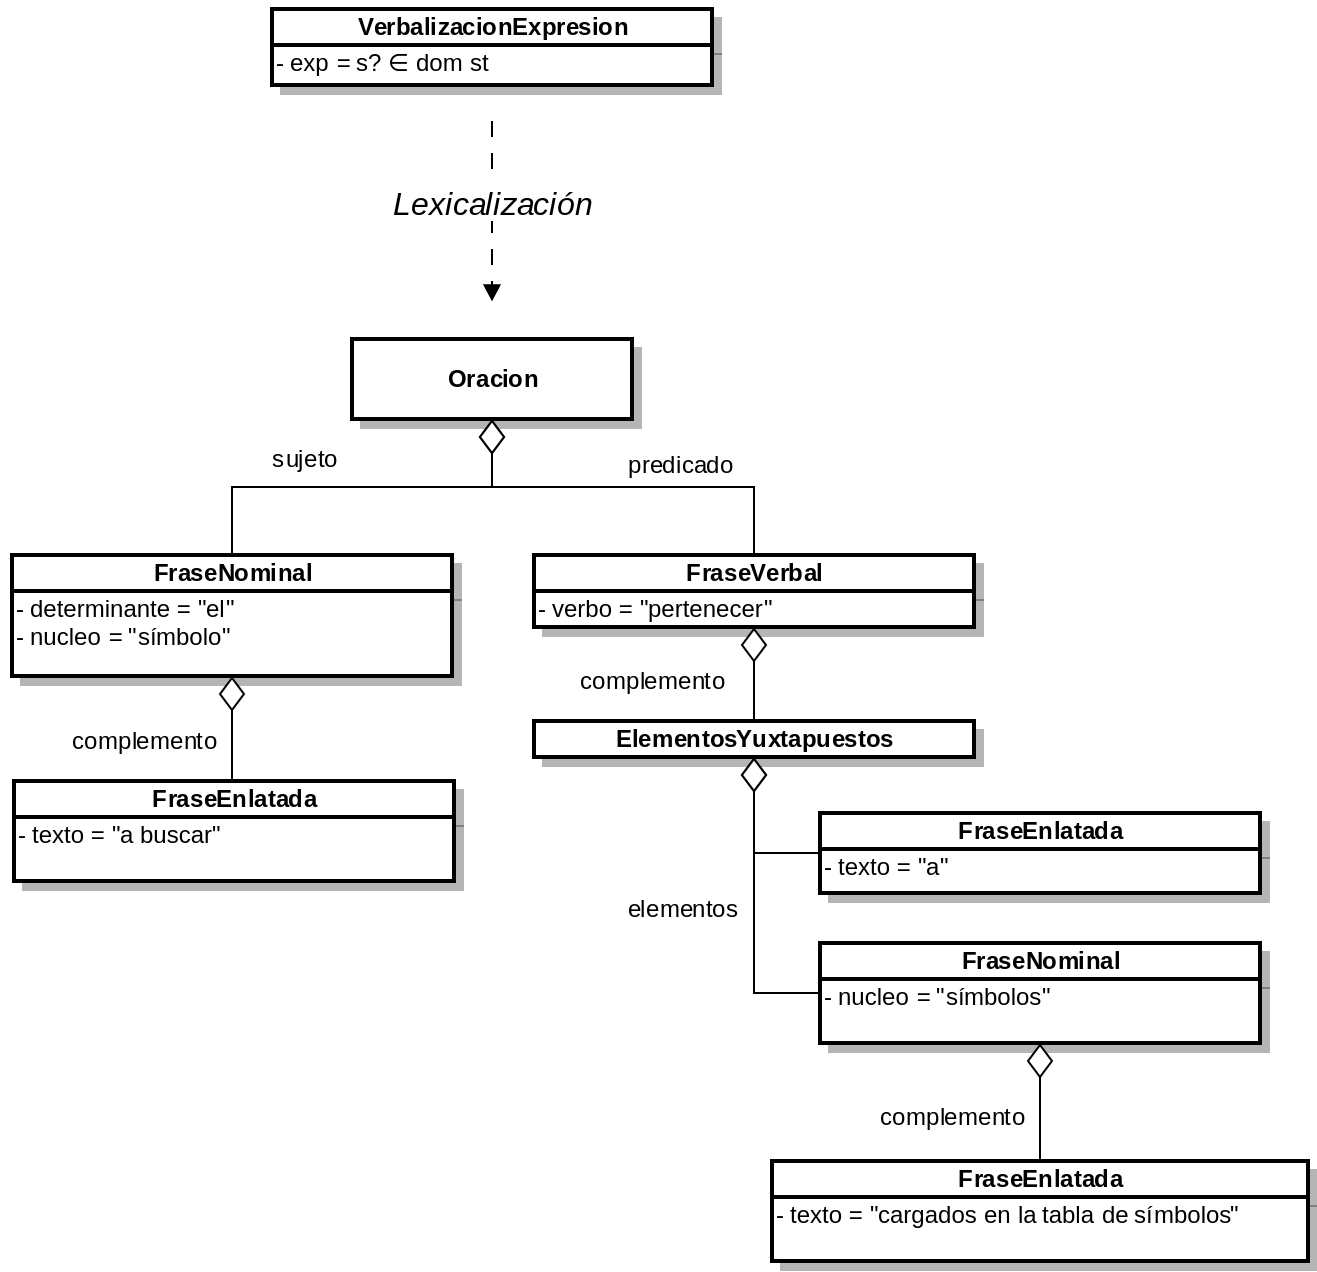
\includegraphics[scale=0.25]{img/phrase_spec_ej.png}
	\caption{Especificación de frase para $s? \protect\in \protect\dom st$.}
  	\label{fig:phase_spec_ej}
\end{figure}

El objetivo del lexicalizador será construir una especificación de frase escogiendo adecuadamente las palabras y constructores sintácticos para siguiente la expresión:

\begin{center}
$s? \in \dom st$
\end{center}

\noindent
Asumimos que contaremos con las siguientes designaciones:

%TODO ver esto
\begin{figure}[H]
\begin{align*} 
  &s? && \approx \text{el símbolo a buscar} \\
  &dom~st && \approx \text{símbolos cargados en la tabla de símbolos}
\end{align*}
\end{figure}

En primer instancia, al no encontrarse designada $s? \in \dom st$ nuestro lexicalizador intentará construir la especificación en base a los operadores que componen la expresión a describir. En el algoritmo \ref{fig:algoritmo_lexicalizacion} incluimos el caso para lexicalizar el predicado $x \in y$ que deberemos utilizar para lexicalizar $s? \in \dom st$. 

Será necesario lexicalizar recursivamente las expresiones: $s?$ y $\dom st$. El resultado de estas lexicalizaciones será usado para construir el sujeto y parte del predicado de la oración a especificar. Estas expresiones se encuentran ambas designadas y por lo tanto su especificación de frase se construirá a partir del texto incluido en sus designaciones. Veremos luego en la siguiente sección la tarea de la función \textsc{designacion} utilizada en el algoritmo anterior encargada de producir una especificación de frase a partir de una expresión designada. 

Como ya mencionamos, utilizaremos el resultado de la lexicalización de $s?$ para formar el sujeto de la oración que deseamos especificar y deberemos luego construir la \emph{FraseVerbal} que cumplirá el rol de predicado. Para construir esta última usaremos la especificación de frase que modelará la verbalización $\dom st$, también mencionada anteriormente. 

Finalmente escogeremos las palabras indicadas a fin de que nuestro sistema pueda dar con una descripción similar a la presentada en el capítulo \ref{sec:corpus_reglas} del análisis de requerimientos. Notemos que para esto utilizamos el verbo ``pertenecer'', en infinitivo, siendo luego tarea del realizador lingüístico la de conjugar el mismo de acuerdo a las reglas gramaticales introducidas en la sección~\ref{sec:corpus_gramatica}. Otra cuestión a mencionar es el uso del elemento \emph{ElementoYuxtapuestos} para salvaguardar la falta de un elemento que nos sirva para modelar un sintagma preposicional en este caso. Nuestro realizador lingüístico deberá procesar los elementos contenidos en cada \emph{ElementoYuxtapuestos} generando un texto resultado de la concatenación de la realización los mismos.

A continuación, en la siguiente sección estudiaremos finalmente, la lexicalización de expresiones designadas.

%TODO cambiar nombre
\section{Lexicalización de expresiones designadas}
\label{sec:verbalizacion_designaciones}
Como vimos en la sección anterior, nuestra tarea de lexicalización deberá hacer uso de las designaciones presentes en la especificación para la construir una especificación de frase. Para esto, cuando una expresión se encuentre designada, nuestro sistema tendrá que procesar la designación, construyendo una especificación de frase que la caracterice. Esto será necesario ya que, como mencionamos previamente, en la etapa de \emph{realización de superficie} nuestro sistema necesitará conocer los distintos constituyentes sintácticos de las oraciones que les provee la especificación de frase y en algunos casos también deberá modificar levemente los textos presentes en las designaciones (por ejemplo, como mencionamos en la sección \ref{sec:corpus_gramatica}, puede ser necesario agregarle el artículo correspondiente a la frase utilizada en la designación).

Para este trabajo, estudiaremos por separado las designaciones parametrizadas y las no parametrizadas.

Comencemos por analizar la lexicalización de una expresión que se encuentra designada por medio de una designación no parametrizada. Por ejemplo, supongamos que queremos construir una especificación de frase para la expresión $s?$ del ejemplo utilizado en la sección anterior. Recordemos que la designación para la misma es:

\begin{center} 
  $s? \approx \text{el símbolo a buscar}$ 
\end{center}

La oración utilizada en la designación anterior, como en los casos observados en el corpus (para designaciones no parametrizadas) resulta un \emph{sintagma nominal}. En este caso ``símbolo'' es el núcleo, ``el'' cumple la función de determinante y ``a buscar'' es el complemento. Será posible entonces, para nuestra tarea de lexicalización, modelar estas frases utilizando una \emph{FraseNominal}. 

Para que nuestro sistema sea capaz de esto deberá analizar sintácticamente las designaciones, \textit{parseando} las mismas con la ayuda de un analizador morfológico que nos permitirá obtener la función sintáctica de cada constituyente de la frase. Además de esto, para simplificar la tarea de \emph{parseo} de nuestro sistema, requeriremos que el usuario escriba las designaciones mediante un sintagma nominal. Es decir, respetando la siguiente estructura:

\begin{figure}[H]
  \centering
   \textbf{Sintagma Nominal} = [\textbf{Determinante}] + \textbf{Núcleo} + [\textbf{Complemento}]
\end{figure}

En el capítulo \ref{cap:implementacion} veremos más en detalle cómo utilizamos un analizador morfológico para ayudarnos con la especificación de las frases incluidas en las designaciones.

Por otro lado, las frases incluidas en las designaciones parametrizadas no poseen la misma estructura. La tarea de modelar minuciosamente estos textos resulta más compleja que para el caso anterior. Por ejemplo, podríamos tener uno o más parámetros presentes dentro del texto, para los cuales deberíamos identificar el rol que cumple cada uno de los anteriores dentro de la oración. Además, nuestro realizador lingüístico sólo soportará oraciones de la forma SVO (sujeto, verbo, objeto) lo cual podría no respetarse en una designación introducida por el usuario. Es por esto que nuestro sistema proveerá solo soporte parcial para las designaciones parametrizadas, aceptando sólo designaciones con un único parámetro. Para describir una expresión parametrizada requeriremos a su vez que el argumento de la misma también se encuentre designado. De esta forma podríamos describir una designación parametrizada de la misma forma que vimos en el capítulo \ref{cap:corpus} reemplazando el parámetro presente en el texto de la designación por el texto incluido en la designación del argumento.

Veamos por ejemplo las siguientes designaciones para una especificación que modela un pequeño sistema de monitoreo de sensores\footnote{Cambiamos el dominio debido a que el ejemplo de la tabla de símbolos no presenta un caso adecuado para ilustrar este problema.} incluido en el corpus (apéndice \ref{ape:corpus}):

\begin{figure}[H]
\begin{align*} 
  &x \in \dom smax && \approx \text{x es un identificador válido} \\
  &s? && \approx \text{el identificador del sensor leído}
\end{align*}
\end{figure}

Donde para describir la expresión $s? \in \dom smax$ bastará con reemplazar el parámetro dentro del texto de la designación parametrizada con el texto incluido en la designación de $s?$ como vemos en la figura \ref{fig:ej_lexicalizacion_desig}.

\begin{figure}[H]
  	\centering
	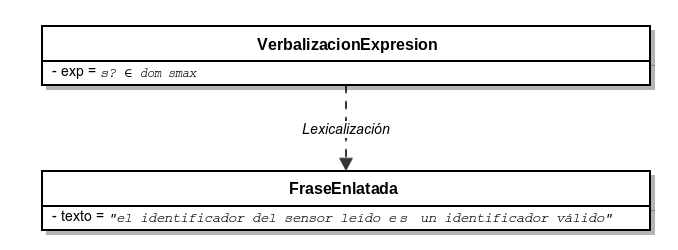
\includegraphics[scale=0.5]{img/ej_lexicalizacion_desig.png}
	\caption{Lexicalización $s? \protect\in \protect\dom smax$.}
  	\label{fig:ej_lexicalizacion_desig}
\end{figure}

Como podemos observar en el ejemplo anterior, al desconocer la estructura del texto presente en las designaciones parametrizadas, deberemos modelar el texto producido por la composición de ambas designaciones utilizando una \emph{FraseEnlatada}. Luego, el texto contenido en estos elementos será realizado sin ningún procesamiento previo, por lo que será responsabilidad del especificador (encargado de escribir las descripciones) que el mismo sea sintáctica y ortográficamente correcto.

\section{Resumen del capítulo}
En este capítulo vimos las tareas necesarias para, partiendo de la salida producida por el \textit{document planner}, constituir una especificación más refinada del texto final. En el próximo capítulo veremos finalmente las tareas que deberán llevarse a cabo para transformar esta especificación del texto en el documento final que contendrá todas las descripciones requeridas por el usuario.

